\documentclass[mathserif]{beamer}
\usepackage{movie15}
\usepackage{psfrag,graphicx}
\usepackage{amsmath}
\usepackage[absolute,overlay]{textpos}

\graphicspath{{figs/}}

\usetheme{Boadilla}
\makeatother
\setbeamertemplate{footline}[frame number]

\usepackage{graphicx}
\usepackage{caption}
\usepackage{subcaption}
\captionsetup{compatibility=false}
\usepackage{amsmath} 
\usepackage{amssymb} 
\usepackage{amsthm}  
\usepackage{bm}
\usepackage{lipsum}
\usepackage[linesnumbered, ruled]{algorithm2e}
\usepackage{color}
\newtheorem{assumption}{Assumptions}
\newtheorem{prop}{Proposition}
\newtheorem{defn}{Definition}
\newtheorem{thm}{Theorem}
\newtheorem{lem}{Lemma}
\newtheorem{cor}{Corollary}
\newtheorem{sol}{Decentralized Solution}
\newtheorem{thresh}{$\epsilon$-thresholding}
\definecolor{light-gray}{gray}{0.8}
\usepackage{textcomp}

\newcommand{\backupbegin}{
   \newcounter{finalframe}
   \setcounter{finalframe}{\value{framenumber}}
}
\newcommand{\backupend}{
   \setcounter{framenumber}{\value{finalframe}}
}
\newcommand{\norm}[1]{\left\lVert #1 \right\rVert}

\makeatletter
\setbeamertemplate{navigation symbols}{}
\title{Class Twenty-Four: Neural Networks}

\author{{ER290: Data, Energy and Justice\\  Instructor: Duncan Callaway} \\
}
\institute{University of California, Berkeley}
\date{Fall 2017}
\begin{document}

\frame{
  \titlepage
}


\begin{frame}{}
\begin{figure}
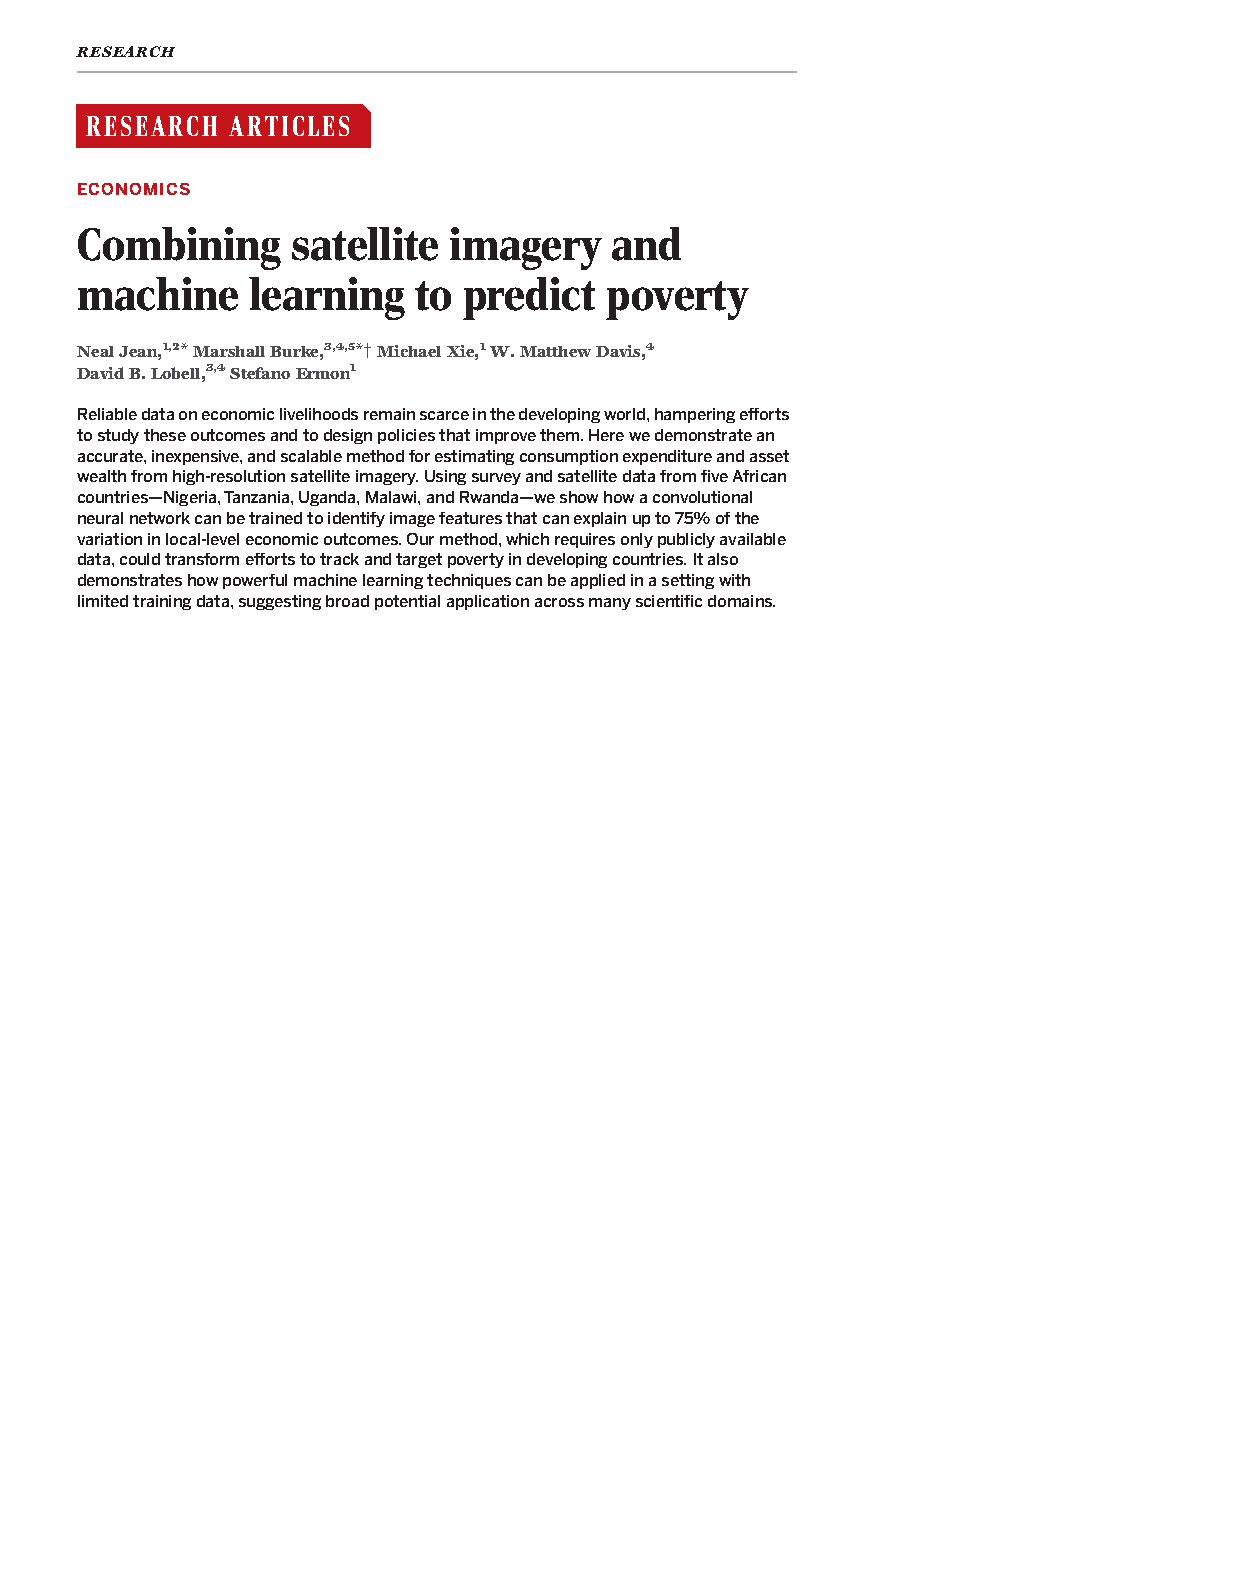
\includegraphics[width=0.7\textwidth]{jean_header}
\caption*{}
\end{figure}
\end{frame}

\begin{frame}{The challenge}

\begin{itemize}
\item International aid agencies want information on where to spend effort
\item Knowing where the poorest people are can inform these decisions
\item But surveying a country's population is expensive, and most survey results are not in the public domain.  
\begin{itemize}
\item About 25\% of African countries did not run any surveys between 2000-2010 from which poverty measures could be computed. 
\end{itemize}
\item Question: can one train a model that uses remote sensing data to predict poverty?
\end{itemize}

\end{frame}

\begin{frame}{Night lights}

\begin{itemize}
\item Some folks have used night satellite imagery to estimate spatial distributions of wealth
\begin{itemize}
\item Basic idea: satellites can see lighting activity at night
\item People with more money use more night lighting.  
\end{itemize}
\item These methods are not accurate at extreme poverty income levels ($<\$1.90$ per person per day)
\item There is little data on extreme poverty (see previous slide) so there isn't a large data set to train models with.
\end{itemize}
\end{frame}

\begin{frame}{Jean \textit{et al's} idea}
\begin{enumerate}
\item Use \textit{daytime }satellite imagery, not night time
\begin{itemize}
\item Landcover type and structures, for example, ought to help to predict poverty.
\end{itemize}
\item Deal with the data paucity problem via ``transfer learning''
\begin{itemize}
\item The idea here is pretty simple: train a neural net on a well known set of images (ImageNet -- labelled data from 1,000 categories, e.g. ``boneshaker'', ``crutch'', ``miniature schnauzer'')

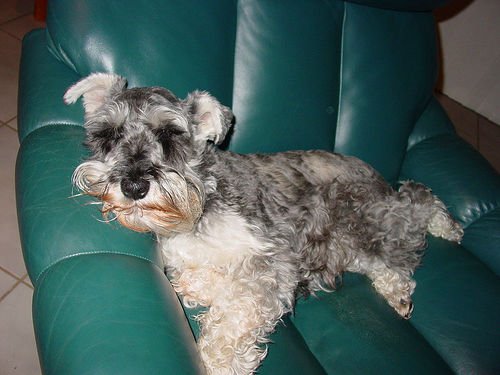
\includegraphics[height=0.3\textheight]{schnauzer} \;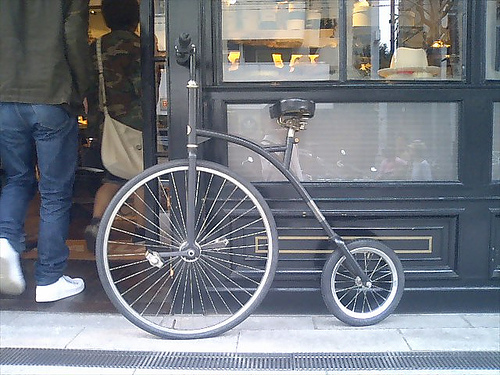
\includegraphics[height=0.3\textheight]{boneshaker}\;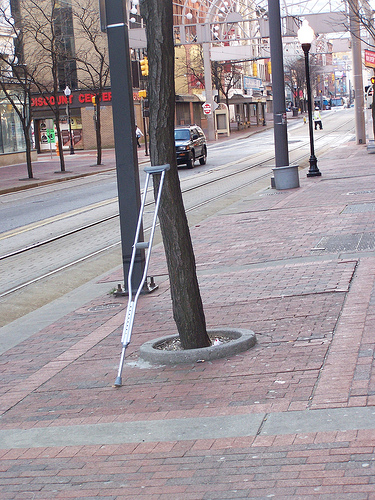
\includegraphics[height=0.3\textheight]{crutch.jpg}

\item the model learns to identify low- level image features such as edges and corners that are common to many vision tasks
\end{itemize}
\end{enumerate}
\end{frame}

\begin{frame}{A bit more on Jean \textit{et al's} transfer learning}
\begin{enumerate}
 \setcounter{enumi}{2}
\item ImageNet-trained model then ``fine tuned'' to use daytime satellite imagery inputs to predict the nighttime light intensities outputs.
\begin{itemize}
\item In doing this Jean\textit{ et al} are falling back on the idea of using night lights (or a prediction of night lights) to measure income and wealth
\item It's desirable to use night lights because it's a globally available data set and is a better proxy for economic activity than the daytime images would be.
\end{itemize}
\item Then use mean cluster-level values from \textit{survey} data (where available) along with the corresponding image features extracted from daytime imagery by the NN are used to train ridge regression models that can estimate cluster-level expenditures or assets.
\begin{itemize}
\item Clusters are geographic areas approximately the size of a village.
\item Survey data approximate hhld expenditures as well as wealth 
\end{itemize}
\end{enumerate}
\end{frame}

\begin{frame}{Basic summary of process}

\begin{itemize}
\item Old: night lights $\rightarrow $ predict wealth and income
\item New: daytime imagery $\rightarrow$ predict night lights $\rightarrow$ predict wealth and income.
\end{itemize}

\end{frame}

\begin{frame}{Wait -- I thought night lights were a lousy proxy for economic activity at low income levels?}

\begin{itemize}
\item Jean \textit{et al} address (or try to address) this head on.  
\item Their claim is that because they're using a linear model (ridge regression) to map day time imagery to  night lights, the model is going to be driven by light-economic relationships at higher income levels.  
\begin{itemize}
 \item If they're lucky, the lower income relationship between \textit{estimated} night lights and economic activity will be decent.
 \end{itemize} 
\end{itemize}
\end{frame}

\begin{frame}{Result - consumption (income) prediction}

\begin{figure}
\includegraphics[width=0.6\textwidth]{jean_fig3}
\caption*{}
\end{figure}
\end{frame}

\begin{frame}{Result - wealth (asset) prediction}

\begin{figure}
\includegraphics[width=0.6\textwidth]{jean_figS3}
\caption*{}
\end{figure}
\end{frame}

\begin{frame}{Some tests}

Their approach:
\begin{itemize}
\item model is on average substantially more predictive of variation in consumption and assets than nightlights alone
\begin{figure}
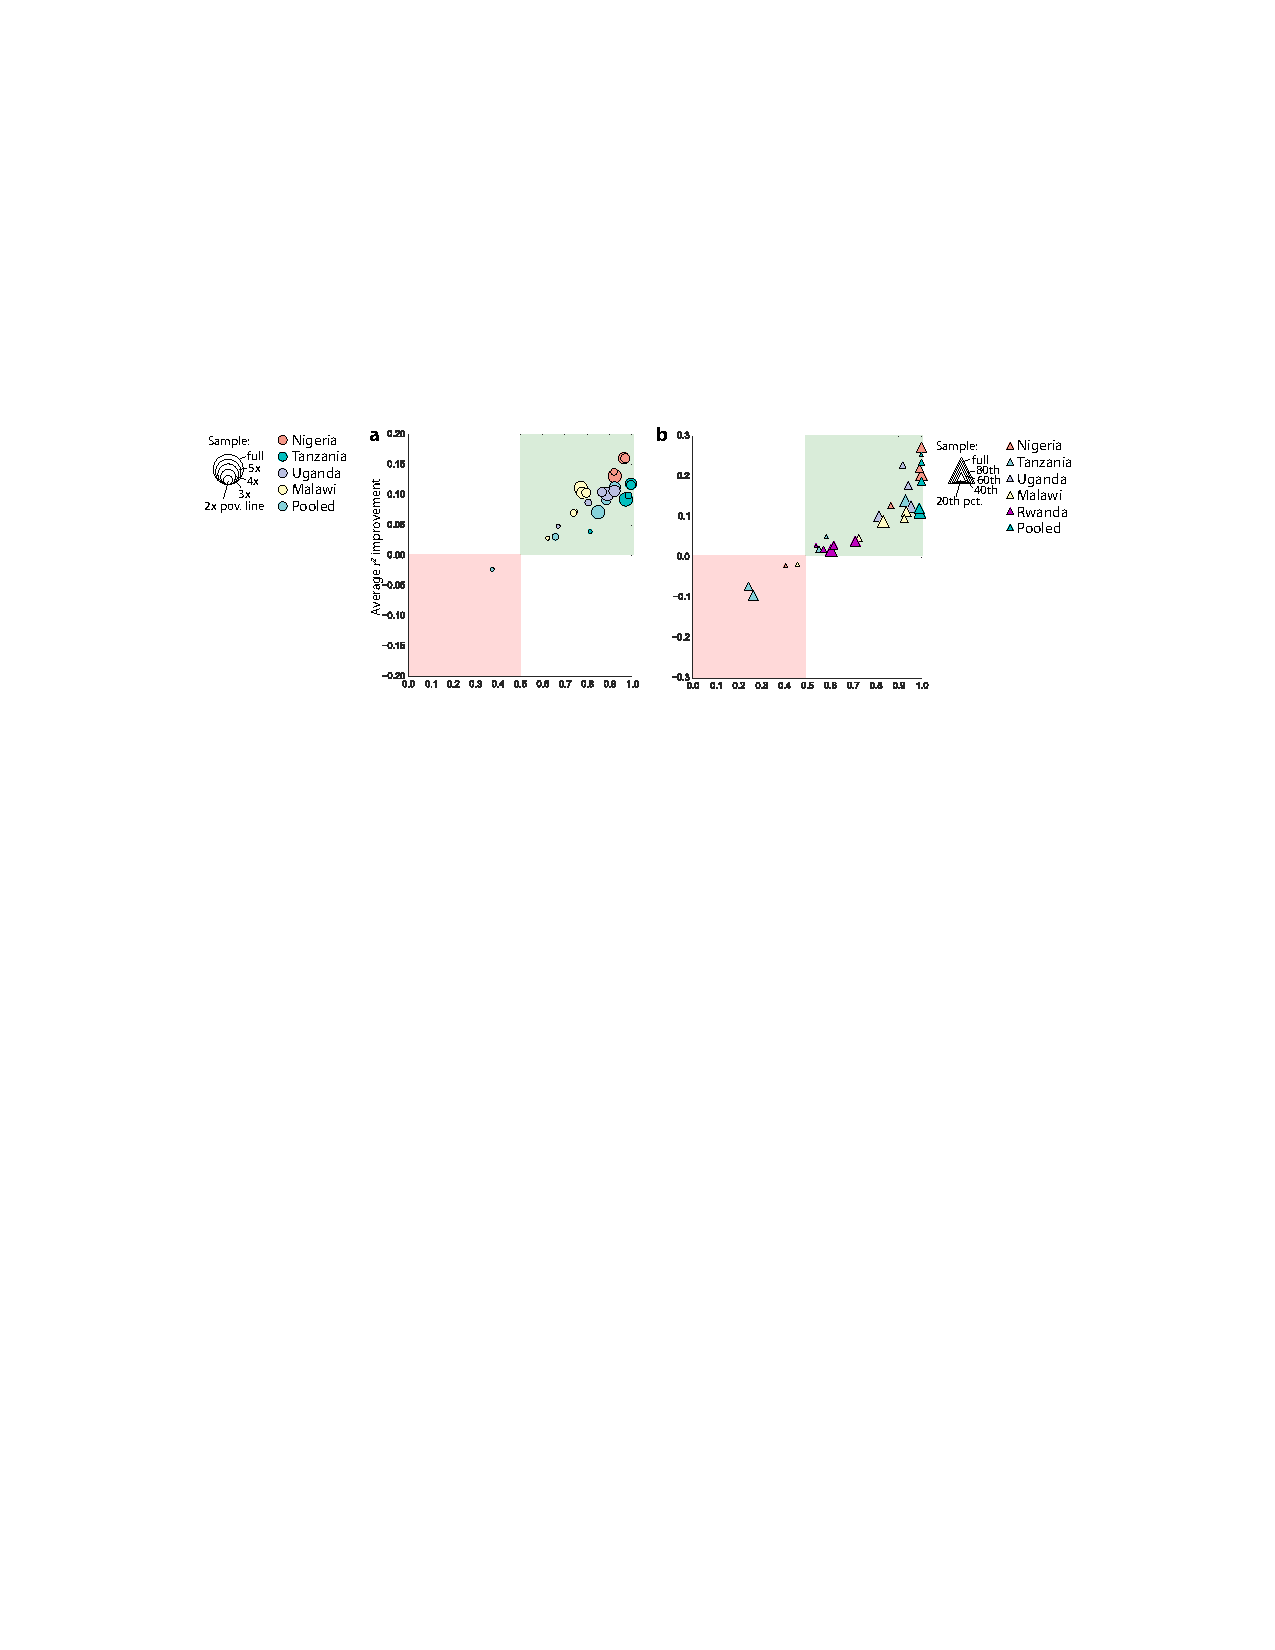
\includegraphics[width=0.8\textwidth]{jean_figS6}
\end{figure}
\item performs as well as or better than an intuitive approach of using data from past surveys to predict outcomes in more recent surveys
\item far outperforms common general-purpose image features such as color histograms
\end{itemize}
\end{frame}

\begin{frame}{A side note on using models trained on one data set to interpret another}

\end{frame}

\begin{frame}{}
\begin{figure}
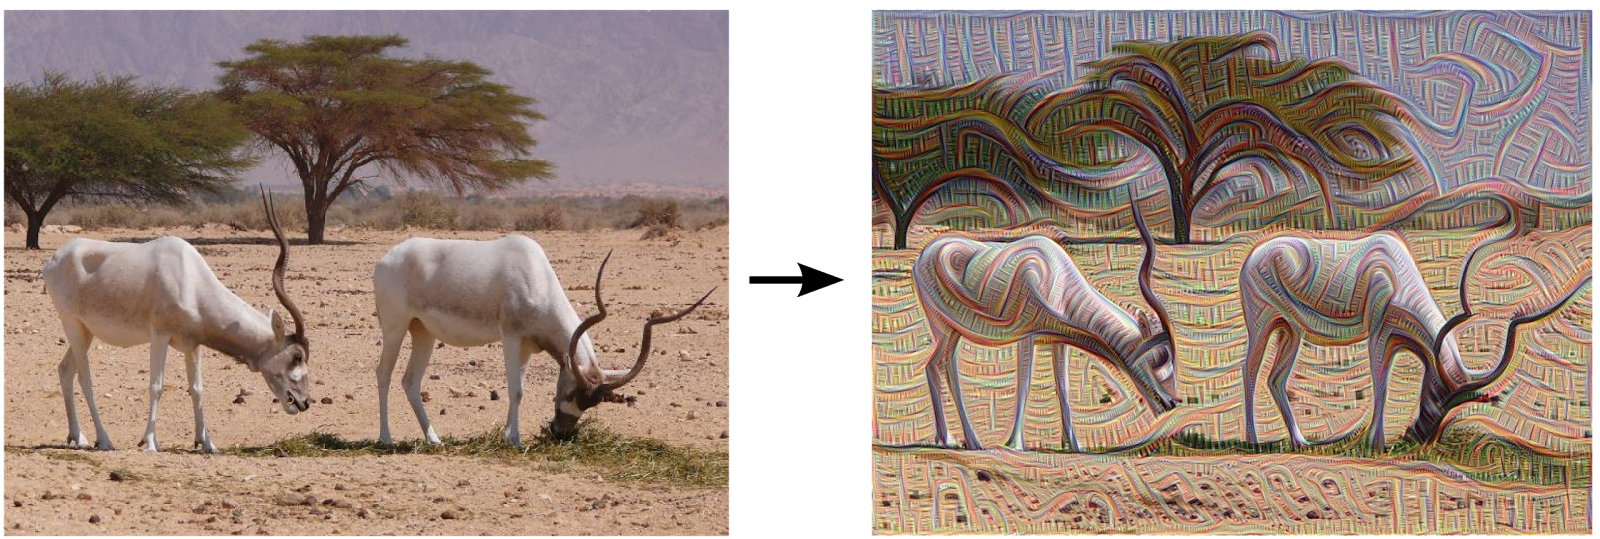
\includegraphics[width=\textwidth]{ibis_google}
\caption*{}
\end{figure}
\end{frame}

\begin{frame}{}
\begin{figure}
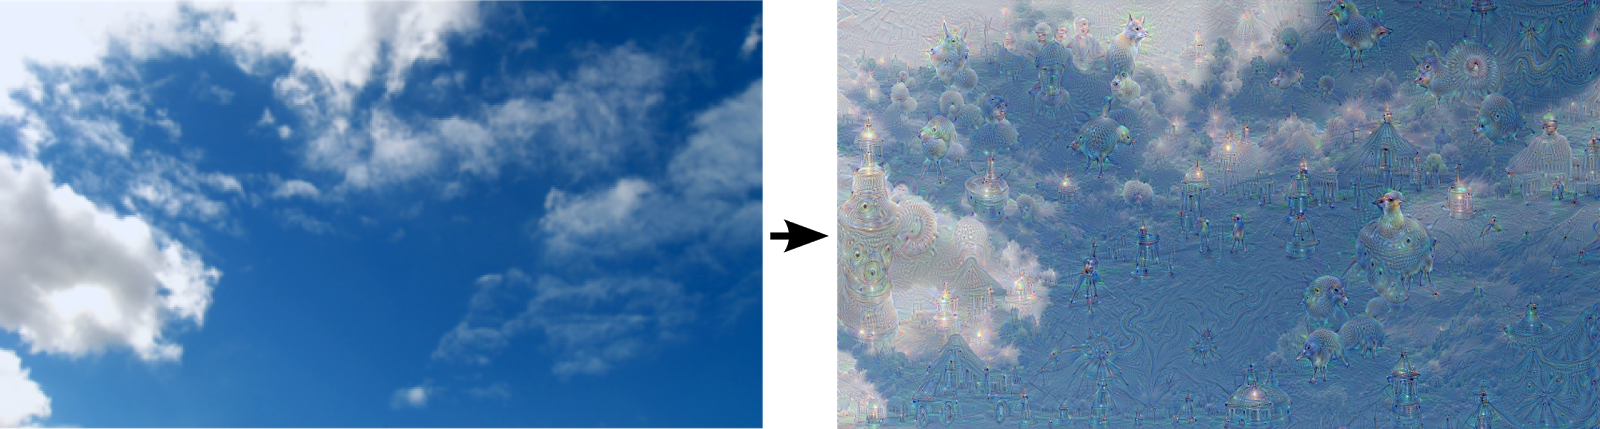
\includegraphics[width=\textwidth]{skyarrow_google}
\caption*{}
\end{figure}
\end{frame}

\begin{frame}{}
\begin{figure}
\includegraphics[width=\textwidth]{funny-animals_google}
\caption*{}
\end{figure}
\end{frame}

\end{document}
